
\subsection{Representing power series}
\begin{frame}
\frametitle{A practical representation for power series}
\begin{lemma}
  Let $f : [0,1] \to \R$ be real analytic.\\
  Then there exists an $l \in \N$ such that 
  $$ \forall x \in [0,1]: \, \left | \frac{f^{(j)}(x)}{j!} \right | \leq 2^l\cdot l^j $$
\end{lemma}
\pause
$l$ can be used to make a tail estimate on
$$ \left | \sum_{n \geq N} a_n z^n \right |  $$
\end{frame}
%\begin{frame}
%\frametitle{Finding $k$ and $A$}
%\begin{itemize}
%\item Choose $k$ appropriately and let $r := \sqrt{k}{2}$
%\item $f_{|z|=r}$ is a continuous function on a compact domain, thus is bounded by some number $A$
%\item By Cauchy Differentiation formula $$|a_n| \leq |\frac{1}{2\pi i}\int_{z=|r|} \frac{f(z)}{|z|^{n+1}} d \lambda| \leq \frac{A}{r^n}$$
%\end{itemize}
%\end{frame}
\begin{frame}[<+->]
\frametitle{Analytic Functions and Computational Complexity}
\begin{theorem}[Kawamura, R\"osnick, M\"uller, Ziegler (2013)]
  The following operators are computable in time polynomial in $n+l$, where $2^{-n}$ is the output precision.
\begin{enumerate}
\item evaluation
\item addition and multiplication
\item differentiation and anti-differentiation
\item parametric maximization
\end{enumerate}
\end{theorem}
\end{frame}
\begin{frame}
\frametitle{Analytic Continuation}
\begin{minipage}{0.45\textwidth}
\begin{center}
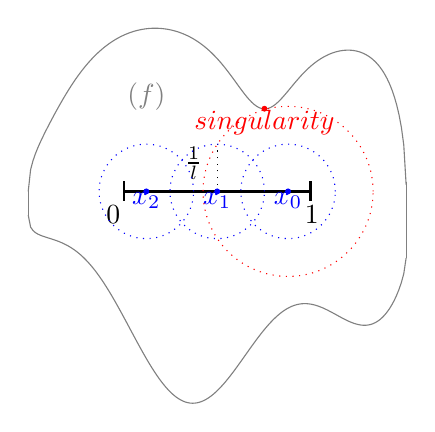
\begin{tikzpicture}[scale=0.6]
%    \draw<3> (-1,1) rectangle (5,-1);
    \node<1->  at (-0.2,-0.5) {$0$};
    \node<1->  at (4.0,-0.5) {$1$};
    \draw<1-> [thick,|-|] (0,0) -- (4,0);
    \node<2->  at (1.5,.6) {$\frac 1{l}$};
    \draw<2->  [dotted] (2.0,0) -- (2.0,1);
    \draw<1-> [domain = 0:8,color=gray] plot[samples=160] (\x-2, {sqrt(16-(\x-4)^2)*(1-1/(\x^2+1) + sin(\x) + (\x/7)^5-\x/6 +1.5- 1/((\x-5)^2+1))/2});
    \draw<1-> [domain = 0:8,color=gray] plot[samples=160] (\x-2, {1/(\x^2+1)/2 + sin(80*\x) + (\x/7)^5-\x/6 -1-sqrt(16-(\x-4)^2)/2});
    \draw<1-> [color=gray] (-2,0) -- (-2,-.5);
    \draw<1-> [color=gray] (6,.19) -- (6,-1.42);
    \node<1-> [color=gray] at (.5,2) {$\dom(f)$};
    \draw<2-> [fill=blue,radius =.05,color=blue] (3.5,0) circle;
    \node<2-> [color=blue] at (3.5,-.2) {$x_0$};
    \draw<2-> [fill=blue,radius =.05,color=blue] (2.0,0) circle;
    \node<2-> [color=blue] at (2.0,-.2) {$x_1$};
    \draw<2-> [radius = 1,color=blue, dotted] (2.0,0) circle; 
    \draw<2-> [fill=blue,radius =.05,color=blue] (0.5,0) circle;
    \node<2-> [color=blue] at (0.5,-.2) {$x_2$}; 
    \draw<2-> [radius = 1,color=blue, dotted] (0.5,0) circle;
    \draw<2-> [radius = 1,color=blue, dotted] (3.5,0) circle;
    \draw<2-> [radius = 1.8, color = red, dotted] (3.5,0) circle; 
    \draw<1-> [fill=red,radius = .05,color = red] (3,1.75) circle;
    \node<1-> [color=red] at (3,1.45) {$singularity$};
\end{tikzpicture}
\end{center}
\end{minipage}
\hfill
\begin{minipage}{0.45\textwidth}
  \onslide<3>{
  The function is uniquely defined by a single germ, i.e., the sequence
  $(\frac{f^{(j)}(x_0)}{j!})_{j \in \N}$ for some $x_0 \in [0,1]$
}
\end{minipage}
\end{frame}

\begin{frame}
\frametitle{Analytic Continuation}
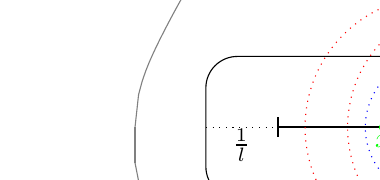
\begin{tikzpicture}[scale=0.9]
    \path [use as bounding box,red] (-100pt,-10pt) rectangle (30pt,40pt);
    \draw[rounded corners=4mm] (-1,1) rectangle (5,-1);
    %\draw (2,0) ellipse (3cm and 1cm);
    \draw [thick,|-|] (0,0) -- (4,0);
    \node at (-.5,-.25) {$\frac 1l$};
    \draw [dotted] (-1,0) -- (0,0);
    \node at (2.2,.5) {$\frac 1l$};
    \draw [dotted] (2,1) -- (2,0);
    \draw [domain = 0:8,color=gray] plot[samples=160] (\x-2, {sqrt(16-(\x-4)^2)*(1-1/(\x^2+1) + sin(\x) + (\x/7)^5-\x/6 +1.5- 1/((\x-5)^2+1))/2});
    \draw [domain = 0:8,color=gray] plot[samples=160] (\x-2, {1/(\x^2+1)/2 + sin(80*\x) + (\x/7)^5-\x/6 -1-sqrt(16-(\x-4)^2)/2});
    \draw [color=gray] (-2,0) -- (-2,-.5);
    \draw [color=gray] (6,.19) -- (6,-1.42);
    \node [color=gray] at (.5,2) {$\dom(f)$};
    \draw<1-3> [fill=blue,radius =.05,color=blue] (3.5,0) circle;
    \node<1-3> [color=blue] at (3.5,-.2) {$x_0$};
    \draw<1-3> [radius = 1,color=blue, dotted] (3.5,0) circle;
    \draw<1-3> [radius = 1.8, color = red, dotted] (3.5,0) circle; 
    \node<2> [color=red] at (2.5,-5) {Check if $x$ in circle};
    \draw [fill=green, radius = .05, color = green] (1.5,0) circle;
    \node [color=green] at (1.5,-.2) {$x$};
    \node<3> [color=red] at (3.0,-5) {Compute Taylor coefficients around $x_1$};
    \draw<3-5> [fill=cyan, radius = .05, color = cyan] (2.75,0) circle;
    \node<3-5> [color=cyan] at (2.75,-.2) {$x_1$};
    \draw<3-5> [radius = 1,color=cyan, dotted] (2.75,0) circle;
    \draw<4-5> [radius = 1.75, color = red, dotted] (2.75,0) circle; 
    \node<4> [color=red] at (2.5,-5) {Check if $x$ in circle};
    \node<5> [color=red] at (3.0,-5) {Compute Taylor coefficients around $x_2$};
    \draw<5-6> [fill=blue, radius = .05, color = blue] (2.25,0) circle;
    \node<5-6> [color=blue] at (2.25,-.2) {$x_2$};
    \draw<5-6> [radius = 1,color=blue, dotted] (2.25,0) circle;
    \draw<6> [radius = 1.85, color = red, dotted] (2.25,0) circle; 
\end{tikzpicture}
\end{frame}
\begin{frame}[<+->]
\frametitle{Computing Taylor coefficients}
\begin{itemize}
  \item The coefficients around some new point $x_0 \in [0,1]$ are given by $c_j := \frac{f^{(j)}(x_0)}{j!}$
  \item $\frac{f^{(d)}(x_0+z)}{d!} = \sum_{j=0}^\infty c_{j+d}\cdot {j+d \choose d}\cdot z^j$
  \item $\left | \sum_{j \geq J} c_{j+d}\cdot {j+d \choose d}\cdot z^j \right | \leq l^d\cdot 2^{l+1-J}(d+1)\cdot {J+d \choose d}$
\end{itemize}
\end{frame}
